\chapter{Implementierung}
\label{ch:implementierung}


\section{Server}
\label{impl:server}
Der Server hat die Aufgabe, die gesamte Kommunikation zwischen Controllern und Robotern zentral zu verwalten und zu koordinieren. Außerdem müssen die Eingabe und Ausgabe der Peripheriegeräte verwaltet, bzw. gesteuert werden. Diese Peripheriegeräte sind die Ladestation, die gefunden werden muss, die Torerkennung, die verarbeitet werden muss und die Infrarot-LED, mithilfe der die Ladestation gefunden werden kann. Auch die Bilddaten, die vom Roboter versendet werden, müssen hier zwischengespeichert werden und anschließend an die Controller weiter gegeben werden.

Als Hostgerät für den Server wurde ein RaspberryPi ausgewählt. Dieser bietet volle Unterstützung für Java-Programme und bietet mit seinen GPIO-Pins eine optimale Basis für die Ansteuerung und Überwachung der Peripheriegeräte. 
Als Programmiersprache wurde Java gewählt.

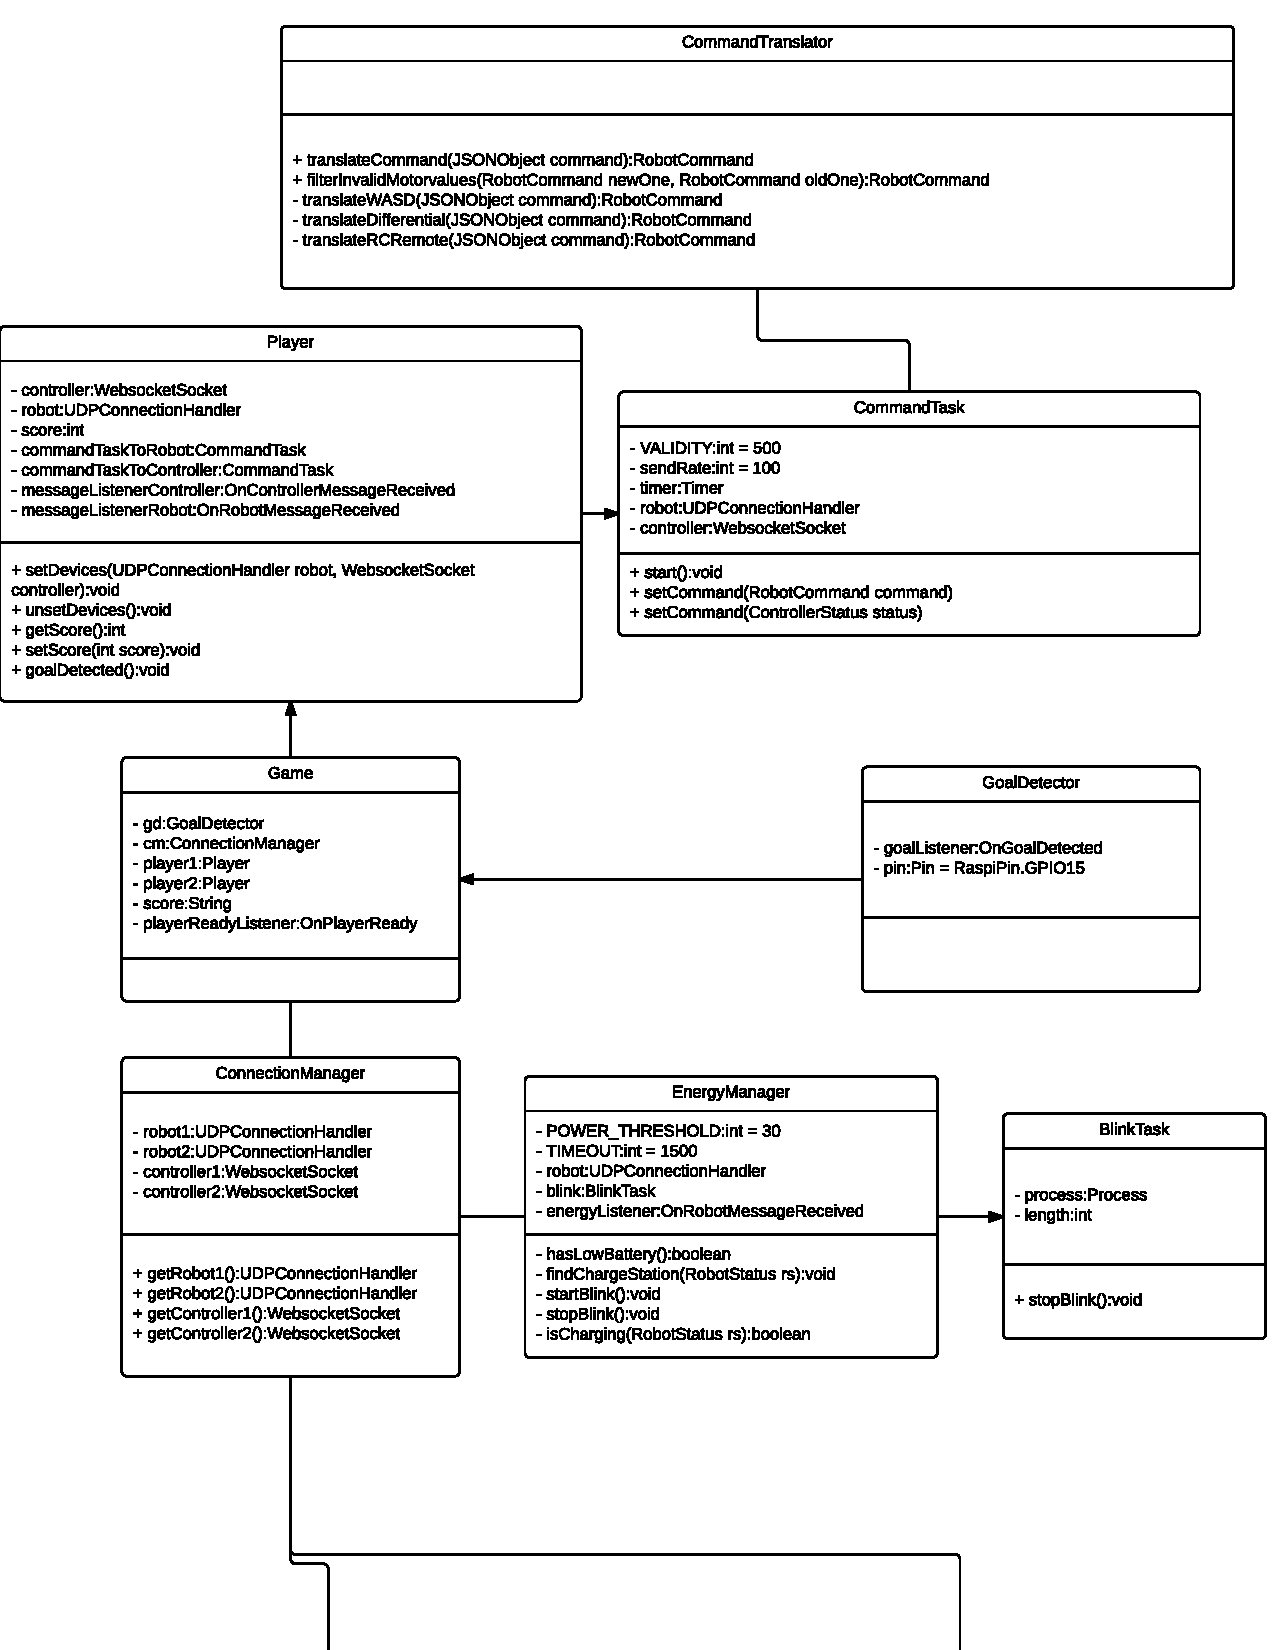
\includepdf[pages={1-}, width=1.2\textwidth]{images/uml_software_all.pdf}

\subsection{Verbindung}
\subsection{Bildübertragung}
\subsection{Torfindung}

\section{Ladestation}
\subsection{Infrarot-LED}
\subsection{Torerkennung}

\section{Webanwendung}

\section{Android-Anwendung}
\subsection{RC-Remote Steuerung}
\subsection{Differential Steuerung}

